\section{Evaluation}

Passive control theory promises a constructive form of robust design with
respect to dynamic stability, and in the presence of network delays and
quantization errors \cite{pass:fettweis86} \cite{ncs:chopra}
\cite{pass:conditions}.  Passive control systems can be constructed from
passive components with the application of a few simple interconnectivity
rules.  Previous work focused on constructive methods includes the approach of
encoding passive interconnections in a modeling language \cite{ncs:mic} or
enforcing passive interconnections at run time using transformations on the data
variables and a data exchange system known as a power junction
\cite{pass:powerjunction}.  

Essentially, a passive component or system introduces no new energy into its
environment.  Output energy is limited to the amount of energy received as
input plus any previously stored energy.  Digital control systems with fast
dynamics (such as the quadrotor) use a zero-order hold to convert control values
produced at discrete time instants into step functions held over a continuous
interval of time.  For certain inputs and state trajectories, the hold process
can introduce small amounts of new energy into the environment.  The sector
bounds analysis proposed by Zames \cite{control:sectors1} can be used to assess
the amount of ``active'' (energy-producing) behavior which we can expect from
our design.

For linear (and some nonlinear) system models, sector bounds may be computed
symbolically during system analysis.  Each component is assigned a real
interval $([a,b] \, -\infty < a \leq b \leq \infty, \, b \geq 0 )$
representing a range of possible input/output behaviors.  Components whose
bounds fall in the interval $[0, \infty]$ are passive (and very close to
stable). Zames also presents rules for computing sector bounds for systems
based on calculated component bounds and different types of interconnections
between components \cite{control:sectors1}.  For our quadrotor system, we
expect the bound $a$ to be small and negative, corresponding to the small
amount of ``active'' behavior due to the hold effects. \cite{quad:passcontrol}
shows a formula for selecting stabilizing gains based on knowledge of the value
of $a$ ($ k < \frac{-1}{a} \, a < 0$).

Empirical verification of the sector bounds is not sound (for all possible
inputs or for discrete time), but can still be a useful technique nonetheless.
Beyond a useful engineering measurement to see whether measured bounds lie
close to the predicted values, if sectors are estimated conservatively
measurements which exceed the bounds are significant.  This indicates that the
selected control gains may not have been sufficient to stabilize the system
with the platform delay effects included in the closed-loop controller.  Our 
test platform is a hardware-in-the-loop simulation environment that allows us to
execute the plant model, and to interface the controller using actual serial links
so that it appears to be a genuine plant with respect to the hardware interface, 
software interface, and timing delays.

\subsection{Passivity, Stability, and Sector Search}

\begin{figure}
\begin{minipage}[b]{0.5\linewidth}
\centering
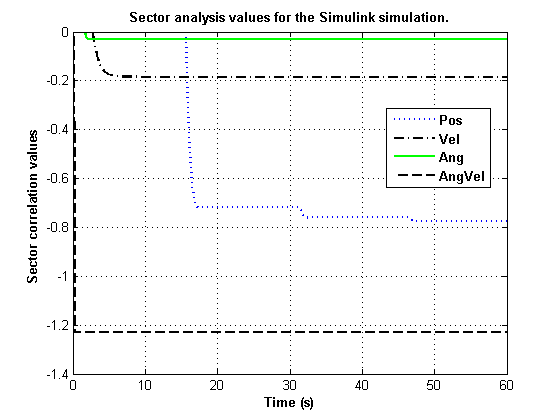
\includegraphics[width=\columnwidth]{figures/simsectors.png}
    \caption{Sector search values for the simulated quad integrator example. }
\end{minipage}
\hspace{0.5cm}
\begin{minipage}[b]{0.5\linewidth}
\centering
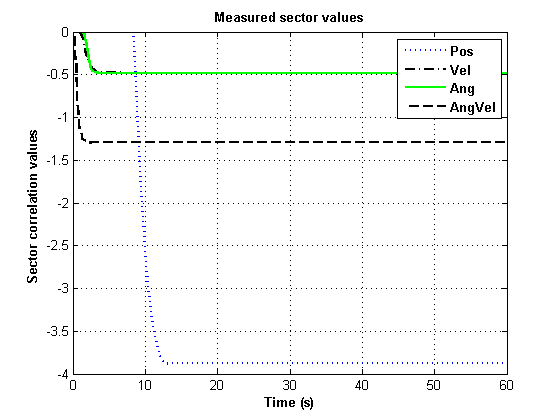
\includegraphics[width=\columnwidth]{figures/meassectors.png}
    \caption{Sector search values for execution on the control platform
(including schedule effects). }
\end{minipage}
    \label{fig:sectors}
\end{figure}

\begin{table}[ht]
\centering

\begin{tabular}[width=\columnwidth]{ | l | l | l | }

\hline
\textbf{Control Signal} & \textbf{Simulated sector values} & \textbf{Measured sector values} \\
\hline \hline
Position & -.7757 & -3.8811 \\
\hline
Velocity & -0.1856 & -0.4830 \\
\hline
Angle & -0.0295 & -0.4831 \\
\hline
Angular Velocity & -1.2292 & -1.2963 \\
\hline
\end{tabular}
\caption{ Sector value comparisons for simulation and execution on the actual platform.}
\label{tab:sectors}
\end{table}

Table \ref{tab:sectors} shows that we have not accounted for all of the effects 
introduced by the platform. Platform effects caused a significant deviation from 
our ideal sector estimates.  
Although the initial platform gains satisfied the sector stability conditions,
the overall system response resulted in significant over-shoot.  After adjusting 
the gains to minimize overshoot, the overall sector estimates were closer
to those for the idealized case but still more negative as would be expected from 
the additional platform effects.  We hope that such sector measures can
be used to better pinpoint sub-platform effects and guide controller tuning.

A more careful review of the data showed that we had
successfully mitigated the delay effects, but differences in the implementation of
single-precision floating-point operations and libraries on three different platforms 
(simulation on x86 vs. actual ARM PXA and ATMega128 with floating-point emulation)
led to some fairly significant differences in behavior.  Section 8.3
below shows the tracking behavior of both the simulation and adjusted controller.

\subsection{Schedulability}

\begin{figure}
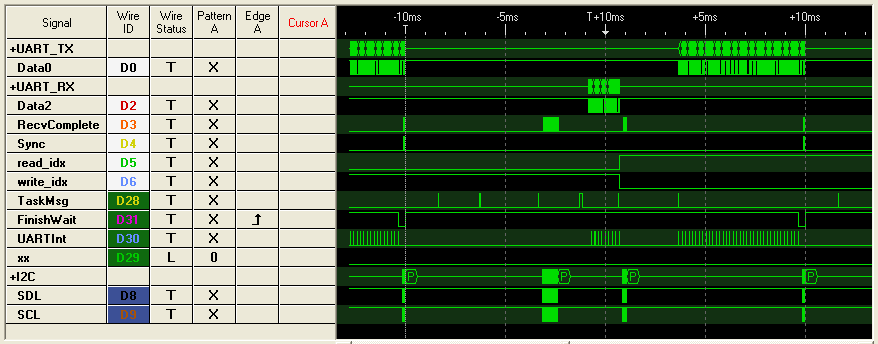
\includegraphics[width=\columnwidth]{figures/probe.png}
    \caption{Timing measurements for the computed schedule. }
    \label{fig:timing}
\end{figure}

Fig. \ref{fig:timing} shows measurements on the ATMega128 (inner loop controller) 
that confirm our schedule calculations.  The running schedule releases tasks and 
transfers messages at the proper times, and that no tasks overrun deadlines.  We 
briefly describe here the signals represented in the figure:

\begin{itemize}
 \item {\bf UART\_TX and Data0} Show the transfer of data from the 
hardware-in-the loop simulator through a serial link to the controller.  The LogicPort
probe interprets the raw signal data (Data0) as an RS-232 exchange (UART\_TX).
 \item {\bf UART\_RX and Data2} Show the transfer of data to the hardware simulator
through the serial link.
 \item {\bf RecvComplete, read\_idx, write\_idx, and UARTInt} Portray various debugging
signals for tracking UART interrupts and double buffering indices.
 \item {\bf Sync} Indicates the start of the hyperperiod.  Each hyperperiod runs for 
20 ms.
 \item {\bf TaskMsg} Contains the start of the message transfers between processors
 as well as the run time of the control tasks.  The tasks start at 4, 7, and 14 ms
from the reference sync pulse.
 \item {\bf I2C, SDL, and SCL} Show the data transfers between processors over
the shared synchronous $I^2C$ bus.  The I2C signal is a protocol-decoded version of the 
raw SDL and SCL data lines.  The small 'P' indicates the end of a message transfer.
Transfers occur at the start of each hyperperiod, and at offsets of 7 and 11 ms.
\end{itemize}

\subsection{Execution Concerns: Reference Tracking}

\begin{figure}
\begin{minipage}[b]{0.5\linewidth}
\centering
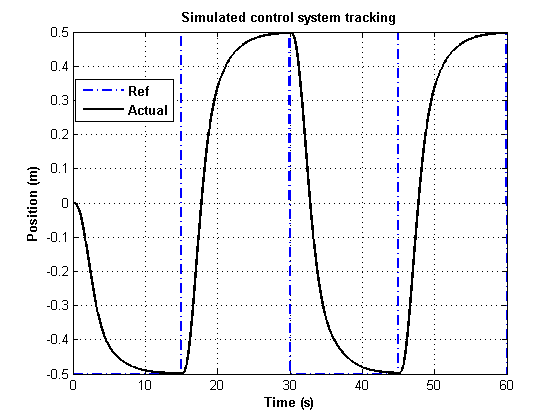
\includegraphics[width=\columnwidth]{figures/tracking.png}
\end{minipage}
\hspace{0.5cm}
\begin{minipage}[b]{0.5\linewidth}
\centering
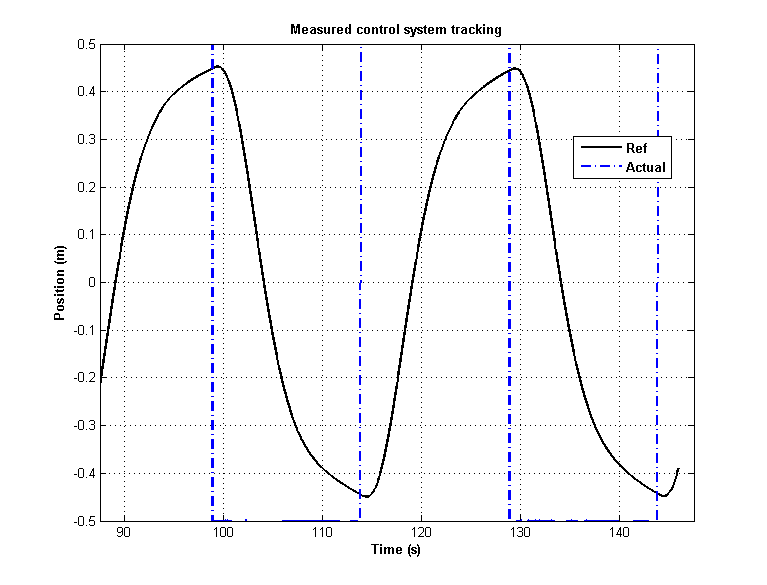
\includegraphics[width=\columnwidth]{figures/measpos.png}
\end{minipage}
   \caption{Square wave input tracking for the simulated quad integrator example and for 
for a hardware-in-the-loop simulation of the actual control platform. }
    \label{fig:exec}

\end{figure}

Fig. \ref{fig:exec} depicts the simulated versus actual position tracking behavior
of the generated control system.  The figure on the right shows the tracking behavior
with the reduced control gains described in Section 8.1.  As expected, the platform
tracking responds more slowly due to delays.
